\documentclass[class=scrartcl, crop=false]{standalone}

\usepackage[sexy]{evan}
\usepackage{nicematrix}
\NiceMatrixOptions{transparent}
\usetikzlibrary{shapes.geometric, calc}


\begin{document}

\section{Isomorphisms}

\begin{definition}
  $(G, \cdot)$ and $(H, \circ)$ are \ul{isomorphic} if there exists a bijection $\phi:G \to H$ such that $\phi(a \cdot b) = \phi(a)\circ\phi(b)$ for all $a, b \in G$.

  Then $\phi$ is an \ul{isomorphism} and we write $G \equiv \sim H$
\end{definition}

\begin{example}
  $\phi:\ZZ_4 \to U_5$ 
  \begin{gather*}
    0 \to 1 \\
    1 \to 2 \\
    2 \to 4 \\
    3 \to 3 \\
    \phi(3 + 2) = \phi(1) = 2 = \phi(3) \cdot \phi(2) = 3 \cdot 4 = 2 \ \checkmark\\
  \end{gather*}

\[
    (\ZZ_4, +): \quad
    \setlength{\extrarowheight}{3pt}% local setting
    \begin{array}{l|*{5}{l}}
    \circ      &0  & 1 & 2 & 3 \\
    \hline
    0          & 0 & 1 & 2 & 3 \\
    1           & 1 & 2 & 3 & 0 \\
    2           & 2 & 3 & 0 & 1 \\
    3           & 3 & 0 & 1 & 2 \\
    \end{array}
\]

\[
    (U_5, \cdot): \quad
    \setlength{\extrarowheight}{3pt}% local setting
    \begin{array}{l|*{5}{l}}
    \circ      &1  &2 & 4 & 3 \\
    \hline
    1          & 1 & 2 & 4 & 3 \\
    2          & 2 & 4 & 3 & 1 \\
    4           & 4 & 3 & 1 & 2 \\
    3           & 3 & 1 & 2 & 4 \\
    \end{array}
\]
  
\end{example}

\begin{note}
  $G$ and $H$ are isomorphic if by "reordering the elements of H", they have the same caylety table - the only difference is notation.

  "bijection between groups extends to a bijection between multiplication tables. Multiplication tables are the same, the difference being notation. A different language"
\end{note}

\begin{example}
  $\phi:\ZZ_4 \to \{\pm 1, \pm i\} \subset \CC^*$

  \begin{gather*}
    0 \to 1 \\
    1 \to i \\
    2 \to -1 \\
    3 \to -i \\\\
    \phi(n) = i^n \\
    \phi(a + b) = i^{a + b} = i^a \cdot i^b = \phi(a) \cdot \phi(b)
  \end{gather*}
\[
    (\{\pm 1, \pm i\} \subset \CC^*, \cdot): \quad
    \setlength{\extrarowheight}{3pt}% local setting
    \begin{array}{l|*{5}{l}}
    \circ      & 1 & i & -1 & -i \\
    \hline
    1           & 1 & i & -1 & -i \\
    i           & i & -1 & -i & 1 \\
    -1           & -1 & -i & 1 & i \\
    -i           & -i & 1 & i & -i \\
    \end{array}
\]
\end{example}

\begin{example}
  $\phi:\ZZ_4 \to \ZZ_4$

   \begin{gather*}
     0 \to 0 \\
     1 \to 3 \\
     2 \to 2 \\
     3 \to 1 \\
  \end{gather*}

  This is an isomorphism.
\end{example}

\begin{theorem}
  $G$ is abelian if and only if the map $\phi: G \to G$ given by $\phi(a) = a^{-1}$ for all $a \in G$ is an isomorphism.
  \begin{proof} .

    ($\Leftarrow$)
    \begin{gather*}
      ba = (a^{-1}b^{-1})^{-1} = \phi(a^{-1}b^{-1}) = \phi(a^{-1})\phi(b^{-1}) = (a^{-1})^{-1}(b^{-1})^{-1} = ab
    \end{gather*}

    ($\Rightarrow$)
    \begin{gather*}
      \phi(a \cdot b) = (ab)^{-1} = b^{-1}a^{-1} = a^{-1}b^{-1} = \phi(a) \cdot \phi(b)
    \end{gather*}
  \end{proof}
\end{theorem}

\begin{example}
  \begin{gather*}
    Q_8 \equiv\sim \left\{
      \pm
      \begin{pmatrix}
        1 & 0 \\
        0 & 1
      \end{pmatrix},
      \pm
      \begin{pmatrix}
        0 & 1 \\
        -1 & 0
      \end{pmatrix},
      \pm
      \begin{pmatrix}
        0 & i \\
        i & 0
      \end{pmatrix},
      \pm
      \begin{pmatrix}
        i & 0 \\
        0 & i
      \end{pmatrix}
    \right\} \\
    Q_8 = \{\pm 1, \pm i, \pm j, \pm k\}
  \end{gather*}
  These two representations of the quaternions are isomorphic to one another.
\end{example}

\begin{example}
  $D_3 \equiv \sim S_3$

  \begin{center}
  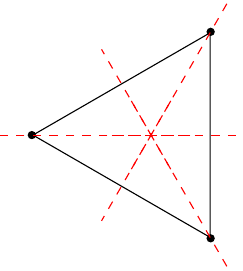
\begin{tikzpicture}[scale=3]
  \def\rps{3} % regular polygon sides
  \node (a) 
  [draw,  blue!0!black,rotate=90,minimum size=3cm,regular polygon, regular polygon sides=\rps] at (0, 0) {}; 

  \foreach \x in {1,2,...,\rps}
    \fill (a.corner \x) circle[radius=.5pt];
    \foreach \x in {1,2,...,\rps}{
    \draw [red,dashed, shorten <=-0.5cm,shorten >=-0.5cm](a.center) -- (a.side \x);
    \draw [red,dashed, shorten <=-0.5cm,shorten >=-0.5cm](a.center) -- (a.corner \x);}

  \end{tikzpicture}
  \end{center}

  \begin{gather*}
    0 \to () \\
    \frac{2\pi}{3} \to \{1 \ 3 \ 2\} \\
    \frac{4\pi}{3} \to \{1 \ 2 \ 3\} \\
    \alpha \to \{2 \ 3\} \\
    \beta \to \{1 \ 2\} \\
    \gamma \to \{1 \ 3\}
  \end{gather*}

  There are many isomorphisms from $D_3$ to $S_3$.
\end{example}

\begin{theorem}
  If $\phi:G \to H$ is an isomorphism, then $\phi^{-1}:H \to G$ is an isomorphism.
  \begin{proof}
    $phi^{-1}$ is a bijection since $\phi$ is ($\phi^{-1}$ exists because $\phi$ is a bijection)

    $\phi^{-1}(a \cdot b) = \phi^{-1}\Big(\phi(\phi^{-1}(a))\phi(\phi^{-1}(b))\Big) = \phi^{-1}\Big(\phi(\phi^{-1}(a)\phi^{-1}(b))\Big) = \phi^{-1}(a)\phi^{-1}(b)$
  \end{proof}
\end{theorem}

\begin{theorem}
  Any "property" of $G$ is a "property" of $H$.
  \begin{example}
    $|G| = |H|$\newline
    $G$ is abelian  $\Leftrightarrow$ $H$ is abelian\newline
    $G$ is cyclic $\Leftrightarrow$ H is cyclic\newline
    $G = \langle g \rangle \Leftrightarrow H = \langle \phi(g) \rangle $
  \end{example}
\end{theorem}

\begin{theorem}
  If $G$ is cyclic and $|G| = \infty$ the $G \equiv \sim \ZZ$ \newline
  If $G$ is cyclic and $|G| = n$ the $G \equiv \sim \ZZ_n$

  \begin{proof}
    Let $G = \langle g \rangle.$ Consider map $\phi:\ZZ \to G$ given by $\phi(i) = g^i$

    Claim that  $\phi$ is a bijection.

    Surjective because each $x \in G$ is $g = g^i$ for some $i$ so $\phi(i) = x$ where x is arbitrary.

    Injective because $\phi(i) = \phi(j) \Rightarrow g^i = g^j \Rightarrow g^i g^{-j} = e \Rightarrow g^{i - j} = e \Rightarrow i = j = 0 \Rightarrow i = j$

    Therefore  $\phi$ is an isomorphism because $\phi(i + j) = g^{i + j} = g^ig^j = \phi(i)\phi(j)$
  \end{proof}
\end{theorem}
  
\end{document}
